\section{Appendix}
\label{sxn:appendix}


In this appendix, we provide more details on several issues that are important for reproducibility of our results.


\subsection{Reproducibility Considerations}


\paragraph{SVD of Convolutional 2D Layers.}

There is some ambiguity in performing spectral analysis on Conv2D layers.  
Each layer is a 4-index tensor of dimension $(w,h,in,out)$, with an $(w\times h)$ filter (or kernel) and $(in, out)$
channels. When $w=h=k$,  giving $(k\times k)$ tensor slices, or \emph{pre-Activation Maps} $\mathbf{W}_{i,L}$ of dimension $(in\times out)$ each. 
%
We identify 3 different approaches for running SVD on a Conv2D layer:
\begin{enumerate}
\item run SVD on each pre-Activation Map $\mathbf{W}_{i,L}$, yielding $(k\times k)$ sets of $M$ singular values
\item stack the maps into a single matrix of, say, dimension $((k\times k\times out)\times in)$, run SVD to get $in$ singular values
\item compute the 2D Fourier Transform (FFT) for each of the $(in, out)$ pairs, and run SVD on the Fourier coeffients~\cite{CNNSVD}, leading to $\sim(k\times in\times out)$ non-zero singular values.
\end{enumerate}
Each method has tradeoffs.  
Method (3) is mathematically sound, but computationally expensive. Method (2) is ambiguous.
For our analysis, because we need thousands of runs, we select method (1), which is the fastest (and is easiest to reproduce).


\paragraph{Normalization of Empirical Matrices.}  

Normalization is an important, if underappreciated, practical issue.
Importantly, the normalization of weight matrices does \emph{not} affect the PL fits because $\alpha$ is scale-invariant.
Norm-based metrics, however, do depend strongly on the scale of the weight matrix---that is the point.
%\nred{Indeed, early theoretical work by Bartlett suggests that the test accuracy depends strongly on the ``total size'' of the weight matrics.}
To apply RMT, we usually define $\mathbf{X}$ with $1/N$ normalization, assuming variance of $\sigma^{2}=1.0$.
%\footnote{For Heavy Tailed theorems, one typically needs a normalization such as \nred{$1/N^{\alpha-1}$. check this}}
Pretrained DNNs are typically initialized with random weight matrices $\mathbf{W}_{0}$, with
 $\sigma^{2}\sim 1/\sqrt{N}$, or some variant, e.g., the Glorot/Xavier normalization~\cite{GloBen10}, or a $\sqrt{2/Nk^2}$ normalization for Convolutional 2D Layers. With this implicit scale, 
we do \emph{not} ``renormalize'' the empirical weight matrices, i.e., we use them as-is.
The only exception is that \emph{we do rescale} the Conv2D pre-activation maps $\mathbf{W}_{i,L}$ 
by $k/\sqrt{2}$ so that they are on the same scale as the Linear / Fully Connected (FC) layers.


\paragraph{Special consideration for NLP models.}

NLP models, and other models with large initial embeddings require special care because the
embedding layers frequently lack the implicit $1/\sqrt{N}$ normalization present in other layers.
For example, in GPT, for most layers, the maximum eigenvalue $\lambda_{max}\sim\mathcal{O}(10-100)$,
but in the first embedding layer, the maximum is of order N (the number of words in the embedding), or
 $\lambda_{max}\sim\mathcal{O}(10^{5})$.  For GPT and GPT2, we treat all layers as-is (although one may to normalize
the first 2 layers by  $\mathbf{X}$ by $1/N$, or to treat them as an outlier).


\subsection{Reproducing Sections \ref{sxn:cv} and \ref{sxn:nlp} }   %% \subsection{Reproducing Sections 4 and 5}

We provide a github repository for this paper that includes Jupyter notebooks that fully reproduce all results (as well as many other results).
All results have been produced using the \emph{WeightWatcher} tool (v0.2.7).
The ImageNet and OpenAI GPT pretrained models are provided in the current 
pyTorch~\cite{pytorch} and Huggingface~\cite{huggingface} distributions, as specified in the \texttt{requirements.txt} file. 

\begin{table}[t]
\small
\begin{center}
\begin{tabular}{|p{1in}|c|}
\hline
Figure & Jupyter Notebook \\
\hline
\ref{fig:vgg-metrics}                                 & WeightWatcher-VGG.ipynb \\
\ref{fig:resnet-accuracy}                             & WeightWatcher-ResNet.ipynb \\
\ref{fig:resnet1k-accuracy}                           & WeightWatcher-ResNet-1K.ipynb \\
\ref{fig:vgg-alpha-layers}                            & WeightWatcher-VGG.ipynb \\
\ref{fig:resnet-alpha-layer}                          & WeightWatcher-ResNet.ipynb \\
\ref{fig:densenet-alpha-layer}                        & WeightWatcher-DenseNet.ipynb \\
\hline
\ref{fig:resnet204D5L}                                & WeightWatcher-Intel-Distiller-ResNet20.ipynb \\
\hline
\ref{fig:GPT-hist}                                    & WeightWatcher-OpenAI-GPT.ipynb \\
\ref{fig:gpt-alpha-layers}, \ref{fig:gpt2-histograms} & WeightWatcher-OpenAI-GPT2.ipynb \\
\hline
\end{tabular}
\end{center}
\caption{Jupyter notebooks used to reproduce all results in Sections~\ref{sxn:cv} and~\ref{sxn:nlp}}
\label{table:notebooks}
\end{table}


\subsection{Reproducing Figure~\ref{fig:resnet204D5L}, for the Distiller Model}

In the \texttt{distiller} folder of our github repo, 
we provide the orginal Jupyter Notebooks, which use the Intel \texttt{distiller} framework.%
\footnote{\url{https://nervanasystems.github.io/distiller}} 
Figure~\ref{fig:resnet204D5L} is from the  \texttt{``...-Distiller-ResNet20.ipynb''} notebook (see Table~\ref{table:notebooks}).  
For completeness, we provide both the results described here, as well as additional results on other pretrained and distilled models using the \emph{WeightWatcher} tool.


\subsection{Reproducing Table~\ref{table:results} in Section~\ref{sxn:all_cv_models} }

In the \texttt{ww-colab} folder of our github repo, we provide several Google Colab notebooks which can be used to reproduce the results of Section~\ref{sxn:all_cv_models}.
The ImageNet-1K and other pretrained models are taken from the pytorch models in the \texttt{omsr/imgclsmob} 
``Sandbox for training convolutional networks for computer vision'' github repository~\cite{osmr}.
The data for each regression can be generated in parallel by running each Google Colab notebook (i.e., \texttt{ww\_colab\_0\_100.ipynb}) simultaneously on the same account.
The data generated are analyzed with \texttt{ww\_colab\_results.ipynb}, which runs all regressions and which tabulates the results presented in Table~\ref{table:results}.

We attempt to run linear regressions for all pyTorch models for each architecture series for all datasets provided.  
There are over $450$ models in all, and we note that the \texttt{osmr/imgclsmob} repository is constantly being updated with new models.
We omit the results for CUB-200-2011, Pascal-VOC2012, ADE20K, and COCO datasets as there are fewer than 15 models for those datasets.  
Also, we filter out regressions with fewer than five datapoints.

We also remove the following outliers, as identified by visual inspection: \texttt{efficient\_b0,\_b2}.
And we remove the entire \texttt{cifar100} \texttt{ResNeXT} series, which is the only example show no trends with the norm metrics.


The final datasets used are shown in Table~\ref{table:datasets}.
The final architecture series used are shown in  Table~\ref{table:architectures}, with the number of models in each.

\begin{table}[t]
\small
\begin{center}
\begin{tabular}{|p{1in}|c|}
\hline
Dataset & $\#$ of Models \\
\hline
imagenet-1k   &  76 \\
svhn          &  30 \\
cifar-100     &  26 \\
cifar-10      &  18 \\
cub-200-2011  &  12 \\
\hline
\end{tabular}
\end{center}
\caption{Datasets used}
\label{table:datasets}
\end{table}

\begin{table}[t]
\small
\begin{center}
\begin{tabular}{|p{2in}|c|}
\hline
Architecture & $\#$ of Models \\
\hline
ResNet                                     & 30 \\
SENet/SE-ResNet/SE-PreResNet/SE-ResNeXt    & 24 \\
DIA-ResNet/DIA-PreResNet                   & 18 \\
ResNeXt                                    & 12 \\
WRN                                        & 12 \\
DLA                                        & 6 \\
PreResNet                                  & 6 \\
ProxylessNAS                               & 6 \\
VGG/BN-VGG                                 & 6 \\
IGCV3                                      & 6 \\
EfficientNet                               & 6 \\
SqueezeNext/SqNxt                          & 6 \\
ShuffleNet                                 & 6 \\
DRN-C/DRN-D                                & 6 \\
ESPNetv2                                   & 6 \\
HRNet                      z                & 6 \\
SqueezeNet/SqueezeResNet                   & 6 \\
\hline
\end{tabular}
\end{center}
\caption{Architectures used}
\label{table:architectures}
\end{table}

\begin{figure}[t]
    \centering
    \subfigure[ImageNet 1K]{
        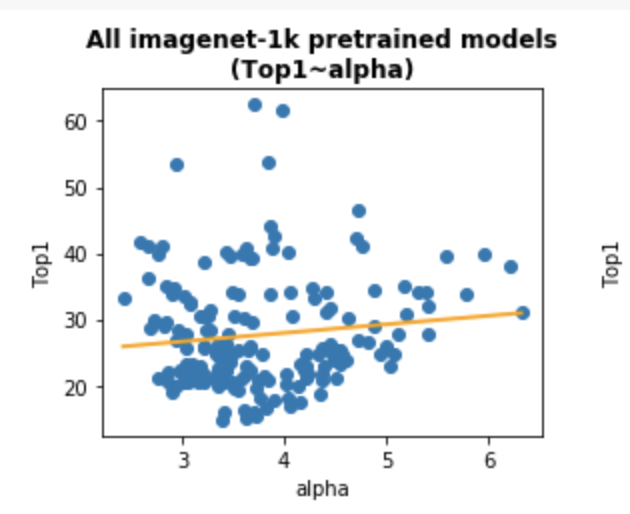
\includegraphics[width=2.5cm]{img/imagenet1k_alpha.png}
        \label{fig:imagenet1k-alpha}
    }
    \qquad
    \subfigure[ CIFAR 10 ]{
        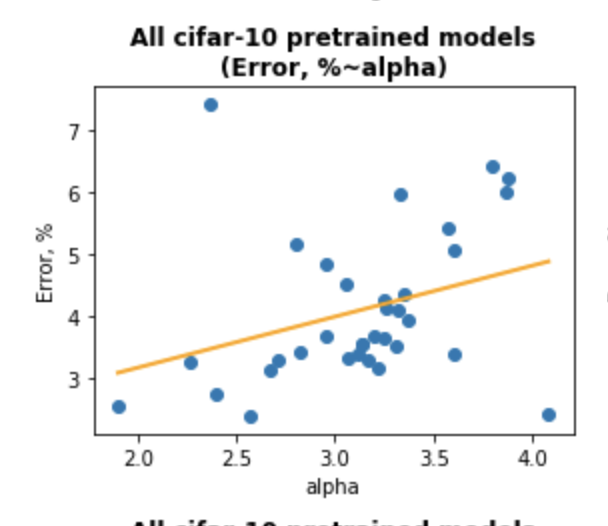
\includegraphics[width=2.5cm]{img/cifar10_alpha.png}
        \label{fig:cifar10.alpha}
    }
    \qquad
    \subfigure[ CIFAR 100 ]{
        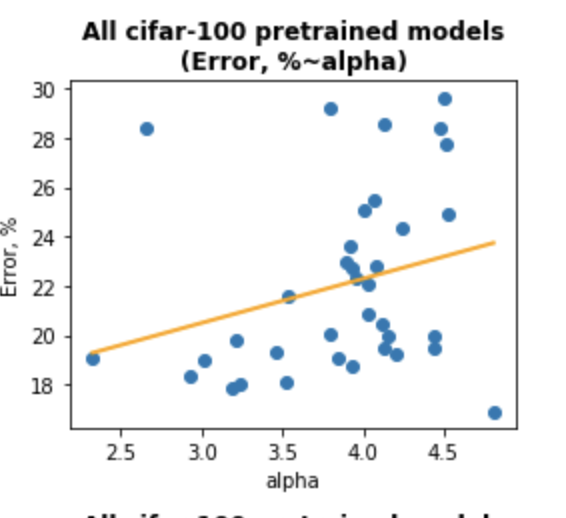
\includegraphics[width=2.5cm]{img/cifar100_alpha.png}
        \label{fig:cifar100.alpha}
    }
    \qquad
    \subfigure[ SVHN ]{
        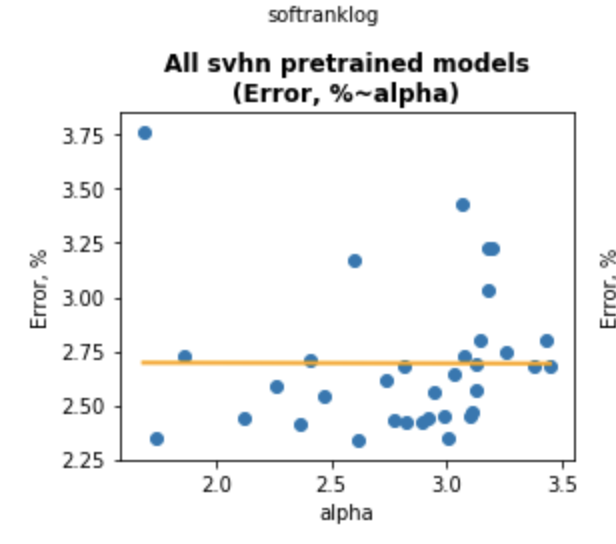
\includegraphics[width=2.5cm]{img/svhn_alpha.png}
        \label{fig:svhn.alpha}
    }
    \qquad
    \subfigure[ CUB 200 ]{
        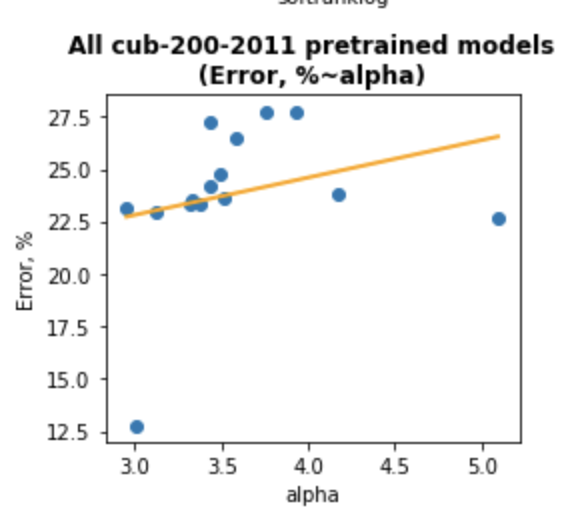
\includegraphics[width=2.5cm]{img/cub200_alpha.png}
        \label{fig:cub200.alpha}
    }
    \caption{\charles{Preliminary charts:} PL exponent $\alpha$ vs. reported Top1 Test Accuracies for pretrained DNNs available\charles{ref} for 5 different data sets.}
    \label{fig:DSalphas}
\end{figure}

To explain further how to reproduce our analysis, we run three batches of linear regressions. 
First, at the global level, we divide models by datasets and run regressions separately on all models of a certain dataset, regardless of the architecture. 
At this level, the plots are quite noisy and clustered, as each architecture has its own accuracy trend; but one can
 still see that most plots show positive relationship with positive coefficients. 
Example regressions are shown in Figure~\ref{fig:DSalphas}, as available in the results notebook.
 
To generate the results in Table~\ref{table:results}, we run linear regressions for each architecture series in Table~\ref{table:architectures}, regressing each empirical Log Norm metric against the reported Top1 (and Top5) errors (as listed on the \texttt{osmr/imgclsmob} github repository README file~\cite{osmr}, with the relevant data extracted and provided in our github repo as \texttt{pytorchcv.html}).
We record the $R^{2}$ and $MSE$ for each metric, averaged over all regressions for all architectures and datasets.
Plots are provided for every regression, and more fine grained results may be computed by the reader by analyzing the data in the \texttt{df\_all.xlsx} file.
The final analysis includes 108 regressions total with 4 or more models, with a positive $R^2$.

\begin{table}[t]
\begin{center}
\begin{tabular}{|c|c|c|c|c|c|}
\hline
Dataset & Model  & $\log\Vert\cdot\Vert_{F}$ & $\log\Vert\cdot\Vert_{\infty}$ & $\hat{\alpha}$ & $\log\Vert\cdot\Vert^{\alpha}_{\alpha}$ \\
\hline
 imagenet-1k & ResNet  & 5.96 &  11.03 & \textbf{3.51} & 4.01 \\
 imagenet-1k & EfficientNet  & 2.67 &  \textbf{1.23} & 2.56 & 2.50 \\
 imagenet-1k & PreResNet  & 6.59 &  15.44 & \textbf{3.59} & 3.71 \\
 imagenet-1k & ShuffleNet  & 35.38 &  89.58 & 19.54 & \textbf{18.48} \\
 imagenet-1k & VGG  & 0.84 &  \textbf{0.68} & 1.89 & 1.59 \\
 imagenet-1k & DLA  & 22.41 &  \textbf{8.49} & 14.69 & 15.68 \\
 imagenet-1k & HRNet  & 0.47 &  0.51 & \textbf{0.16} & 0.16 \\
 imagenet-1k & DRN-C  & 0.60 &  0.66 & \textbf{0.40} & 0.48 \\
 imagenet-1k & SqueezeNext  & 21.94 &  21.39 & 13.31 & \textbf{13.23} \\
 imagenet-1k & ESPNetv2  & 13.77 &  14.74 & \textbf{1.87} & 2.53 \\
 imagenet-1k & IGCV3  & 1.94 &  87.76 & 8.48 & \textbf{1.09} \\
 imagenet-1k & ProxylessNAS  & \textbf{0.19} &  0.26 & 0.28 & 0.26 \\
 imagenet-1k & SqueezeNet  & 0.11 &  0.11 & \textbf{0.07} & 0.08 \\
\hline
 cifar-10 & ResNet  & 0.31 &  0.30 & \textbf{0.28} & 0.28 \\
 cifar-10 & DIA-ResNet  & \textbf{0.05} &  0.08 & 0.28 & 0.32 \\
 cifar-10 & SENet  & 0.09 &  0.09 & \textbf{0.04} & 0.04 \\
\hline
 cifar-100 & ResNet  & 4.13 &  4.50 & \textbf{3.06} & 3.06 \\
 cifar-100 & DIA-ResNet  & \textbf{0.36} &  1.38 & 0.93 & 1.02 \\
 cifar-100 & SENet  & 0.36 &  0.43 & \textbf{0.26} & 0.26 \\
 cifar-100 & WRN  & 0.14 &  0.20 & 0.07 & \textbf{0.06} \\
\hline
 svhn & ResNet  & 0.04 &  0.04 & \textbf{0.02} & 0.02 \\
 svhn & DIA-ResNet  & 0.00 &  \textbf{0.00} & 0.02 & 0.02 \\
 svhn & SENet  & \textbf{0.00} &  0.00 & 0.00 & 0.00 \\
 svhn & WRN  & 0.01 &  0.01 & 0.01 & \textbf{0.01} \\
 svhn & ResNeXt  & 0.00 &  \textbf{0.00} & 0.01 & 0.01 \\
\hline
 cub-200-2011 & ResNet  & 0.20 &  \textbf{0.18} & 3.19 & 3.21 \\
 cub-200-2011 & SENet  & \textbf{1.07} &  1.29 & 1.85 & 1.95 \\
\hline
\end{tabular}
\end{center}
\caption{MSE Results for all CV model regressions. }
\label{table:MSEresults}
\end{table}





\begin{table}[t]
\begin{center}
\begin{tabular}{|c|c|c|c|c|c|}
\hline
Dataset & Model  & $\log\Vert\cdot\Vert_{F}$ & $\log\Vert\cdot\Vert_{\infty}$ & $\hat{\alpha}$ & $\log\Vert\cdot\Vert^{\alpha}_{\alpha}$ \\
\hline
imagenet-1k & ResNet  & 0.82 &  0.67 & \textbf{0.90} & 0.88 \\
 imagenet-1k & EfficientNet  & 0.65 &  \textbf{0.84} & 0.67 & 0.67 \\
 imagenet-1k & PreResNet  & 0.73 &  0.36 & \textbf{0.85} & 0.85 \\
 imagenet-1k & ShuffleNet  & 0.63 &  0.06 & 0.80 & \textbf{0.81} \\
 imagenet-1k & VGG  & 0.71 &  \textbf{0.76} & 0.35 & 0.45 \\
 imagenet-1k & DLA  & 0.13 &  \textbf{0.67} & 0.43 & 0.39 \\
 imagenet-1k & HRNet  & 0.91 &  0.90 & \textbf{0.97} & 0.97 \\
 imagenet-1k & DRN-C  & 0.81 &  0.79 & \textbf{0.87} & 0.85 \\
 imagenet-1k & SqueezeNext  & 0.05 &  0.07 & 0.42 & \textbf{0.43} \\
 imagenet-1k & ESPNetv2  & 0.42 &  0.38 & \textbf{0.92} & 0.89 \\
 imagenet-1k & IGCV3  & 0.98 &  0.12 & 0.92 & \textbf{0.99} \\
 imagenet-1k & SqueezeNet  & 0.01 &  0.00 & \textbf{0.38} & 0.26 \\
 imagenet-1k & ProxylessNAS  & \textbf{0.68} &  0.56 & 0.53 & 0.58 \\
\hline
 cifar-10 & ResNet  & 0.58 &  0.59 & \textbf{0.62} & 0.61 \\
 cifar-10 & DIA-ResNet  & \textbf{0.96} &  0.93 & 0.74 & 0.71 \\
 cifar-10 & SENet  & 0.91 &  0.91 & \textbf{0.96} & 0.96 \\
\hline
 cifar-100 & ResNet  & 0.61 &  0.58 & \textbf{0.71} & 0.71 \\
 cifar-100 & DIA-ResNet  & \textbf{0.96} &  0.85 & 0.90 & 0.89 \\
 cifar-100 & SENet  & 0.97 &  0.96 & \textbf{0.98} & 0.98 \\
 cifar-100 & WRN  & 0.32 &  0.04 & 0.66 & \textbf{0.69} \\
\hline
 svhn & ResNet  & 0.69 &  0.70 & \textbf{0.82} & 0.81 \\
 svhn & DIA-ResNet  & 0.94 &  \textbf{0.95} & 0.78 & 0.77 \\
 svhn & SENet  & \textbf{0.99} &  0.96 & 0.98 & 0.98 \\
 svhn & WRN  & 0.13 &  0.10 & 0.20 & \textbf{0.21} \\
 svhn & ResNeXt  & 0.87 &  \textbf{0.90} & 0.64 & 0.75 \\
\hline
 cub-200-2011 & ResNet  & 0.94 &  \textbf{0.95} & 0.08 & 0.08 \\
 cub-200-2011 & SENet  & \textbf{0.66} &  0.59 & 0.41 & 0.38 \\
\hline
\end{tabular}
\end{center}
\caption{$R^{2}$ Results for all CV model regressions. }
\label{table:R2results}
\end{table}
